\documentclass{alex_hü}

\name{Alexander Helbok}
\course{PS Physik}
\hwnumber{3}


\begin{document}
\renewcommand{\labelenumi}{\alph{enumi})}


\begin{mybox}{1. Potentialverlauf einer geladenen Hohlkugel}
	\centering \( k = \tfrac{1}{4\pi \epsilon_0}, V = \int\limits_{V_i}^{\infty}\ \vec{E}\ \mathrm{d}\vec{s} \)
	\tcblower
		\boxed{
			\begin{aligned}
				E(r) = \begin{cases}
					0& \quad $for $\ 0 < r \le R_i, \\
					\tfrac{kQ}{R_a^3-R_i^3} \left(r - \tfrac{R_i^3}{r^2}\right)& \quad $for $\ R_i < r < R_a, \\
					kQ \tfrac{1}{r^2}& \quad $for $\ R_a \le r. 
				\end{cases} 
			\end{aligned}
		}\\[2em]
		\underline{For  \(R_a \leq r\):}
		\begin{flalign*}
			E(r) &= kQ \tfrac{1}{r^2} &&\\
			V_1(r) &= \uint[r,\infty]{\vec{E}(r)}{r} = kQ \uint[r,\infty]{\tfrac{1}{r^2}}{r} = kQ \tfrac{1}{R_a} &&\\
			V_1(r) &= kQ \tfrac{1}{r} &&\\
		\end{flalign*}
		\underline{For \(R_i < r < R_a\):}
		\begin{flalign*}
			E(r) &= \tfrac{kQ}{R_a^3-R_i^3} \left(r - \tfrac{R_i^3}{r^2}\right) &&\\
			V_2(r) &= \uint[r,\infty]{\vec{E}(r)}{\vec{r}} = kQ\left( \uint[r,R_a]{\tfrac{r^3 - R_i^3}{r^2(R_a^3-R_i^3)}}{r} + \tikzmark{1} \uint[R_a,\infty]{\tfrac{1}{r^2}}{r} \tikzmark{2} \right)  = &&\\[2em]
			&= kQ\left( -\tfrac{r^3R_a - rR_a^3 + 2 rR_i^3 + 2R_aR_i^3}{2rR_a^4 - 2rR_aR_i^3} + \tfrac{1}{R_a} \right)  &&\\[2em]
			V_2(r) &= -kQ\frac{r^3-3rR_a^2 + 2 R_i^3}{2rR_a^3 - 2rR_i^3} &&\\
		\end{flalign*}
		\AddUnderBrace[2.2em]{1}{2}{$= V_1(R_a)$}
		\newpage
		\underline{For \( r \leq R_i\):}
		\begin{flalign*}
			E(r) &= 0 &&\\
			V_3(r) &= \uint[r,\infty]{\vec{E}(r)}{\vec{r}} = kQ\left(\tikzmark{5} \uint[r,R_i]{0}{r} \tikzmark{6} + \tikzmark{3} \uint[R_i,\infty]{\tfrac{r^3 - R_i^3}{r^2(R_a^3-R_i^3)}}{r} \tikzmark{4} \right) = &&\\[2em]
			V_3(r) &= -kQ\frac{3 (R_a+R_i)}{2 (R_a^2+R_a R_i+R_i^2)} &&\\
		\end{flalign*}
		\AddUnderBrace[2.2em]{3}{4}{$= V_2(R_i)$}
		\AddUnderBrace[2.2em]{5}{6}{$= 0$}
		\boxed{
			\begin{aligned}
				V(r) = \begin{cases}
					-kQ\frac{3 (R_a+R_i)}{2 (R_a^2+R_a R_i+R_i^2)}& \quad $for $\ 0 < r \le R_i, \\[1.5ex]
					-kQ\frac{r^3-3rR_a^2 + 2 R_i^3}{2rR_a^3 - 2rR_i^3}& \quad $for $\ R_i < r < R_a, \\[1.5ex]
					kQ \tfrac{1}{r}& \quad $for $\ R_a \le r. 
				\end{cases} 
			\end{aligned}
		}\\[2cm]
		\begin{tikzpicture}
			\begin{axis}[
				width=350pt,
				height=250pt,
				axis lines=center,
				%y axis line style={thick},
				tick align=outside,
				xmin=0,xmax=14,ymin=0,ymax=0.45,
				xlabel style={below},
				xtick = {2,4}, ytick = {0.321},
				xticklabels={\( R_i \), \( R_a \)},
				yticklabels={\( V_{max} \)},
				xlabel=$r$,
				ylabel=$V$,
				grid=major,
				grid style={thin,densely dotted,black!20},
				%legend columns=2,
				legend style={at={(axis description cs:1,0.35)},anchor=east}]
				\addplot [-, thick,  blue, domain = 4:14, smooth] {1/x};
				\addplot [-, thick,  blue, domain = 2:4, smooth] {-(x^3 - 48*x + 16)/(128*x - 16*x)};
				\addplot [-, thick,  blue, domain = 0:2, smooth] {-(2^3 - 48*2 + 16)/(128*2 - 16*2)};
			\end{axis}
		\end{tikzpicture}\\
\end{mybox}

\begin{mybox}{2. Elektrisches Feld und Potential eines geladenen Stabes}
	\centering \( k = \tfrac{1}{4\pi \epsilon_0};\quad \mathrm{d}Q = \lambda \mathrm{d}z;\quad d = \sqrt{r_P^2 + (z_P - z)^2} \)
	\tcblower
	\begin{enumerate}
		\item 
		\begin{flalign*}
			\mathrm{d}V &= k\tfrac{1}{d}\ \mathrm{d}Q = k\lambda \tfrac{1}{\sqrt{r_P^2 + (z_P - z)^2}}\ \mathrm{d}z &&\\
			V &= k\lambda \int\limits_{-l/2}^{l/2}\ \tfrac{1}{\sqrt{r_P^2 + (z_P - z)^2}}\ \mathrm{d}z = &&\\
			&= \dl{k\lambda\ln \left(\frac{\sqrt{\left( \tfrac{l}{2}+z_P \right)^2 + r_P^2} + \tfrac{l}{2}+z_P}{\sqrt{\left( -\tfrac{l}{2}+z_P \right)^2 + r_P^2} - \tfrac{l}{2}+z_P }\right)} &&
		\end{flalign*}
		\tcbline
		\item \( z_P = 0;\quad r_P = x_P;\quad l \ll x_P \)
		\begin{flalign*}
			V &= k\lambda\ln \left(\frac{\sqrt{l^2 + 4r_P^2} + l}{\sqrt{l^2 + 4r_P^2} - l}\right) &&\\
			&= k\lambda\ln \left(\frac{\sqrt{l^2 + 4x_P^2} + l}{\sqrt{l^2 + 4x_P^2} - l}\right) &&\\
			&\approx k\lambda\ln\left(\frac{2x_P + l}{2x_P - l}\right) \approx k\lambda \ln(1) &&\\
			&= \dl{0} &&
		\end{flalign*}
		\hfill
		\begin{minipage}[t]{0.3\textwidth}
			\vspace{-4cm}
			\boxed{
				\begin{aligned}
					\sqrt{l^2 + 4x_P^2} &\approx 2x_P \\
					2x_P \pm l &\approx 2x_P
				\end{aligned}
			}
		\end{minipage}\\
	\end{enumerate}
\end{mybox}
\newpage
\begin{mybox}{3. Elektrische Ladung zwischen Kugelladungen}
	\centering \( k = \tfrac{1}{4\pi \epsilon_0} \)
	\tcblower
	\begin{enumerate}
		\item \( \vec{F} = \vec{E}_2(9.5d) * q = \dl{k \tfrac{qQ}{(9.5d)^2} \vector{1\\ 0\\ 0}} \)
		\tcbline
		\item
		\begin{minipage}{\textwidth}
			\hspace{1cm}
			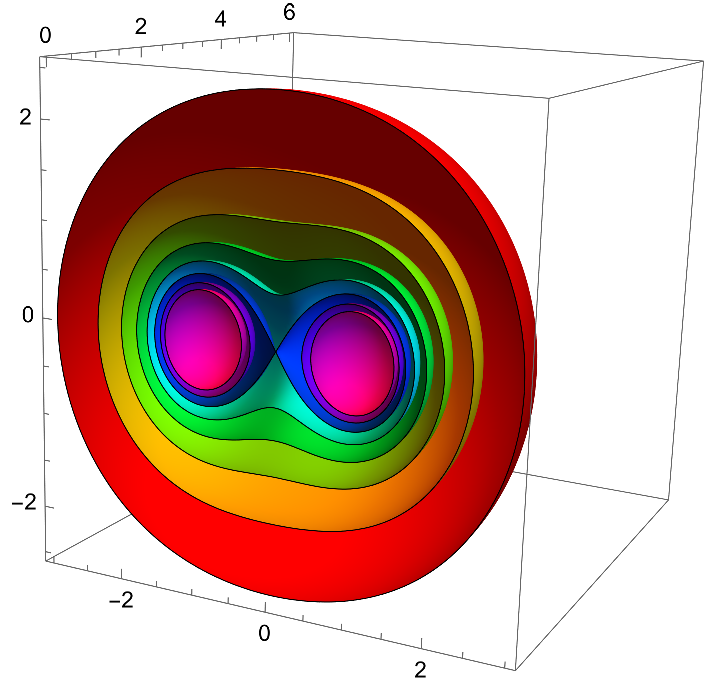
\includegraphics[scale=0.7]{4.pdf}
		\end{minipage}\vspace{0.5cm}
		\tcbline
		\item 
		\begin{flalign*}
			K &= W &&\\
			\tfrac{1}{2}mv^2 &= \uint[9.5d,9d]{\vec{F}}{\vec{r}} = kqQ\left( \tfrac{1}{9.5d} - \tfrac{1}{9d}\right)  = kqQ \tfrac{1}{171d} &&\\
			v &= \dl{\sqrt{\tfrac{2kqQ}{171dm}}} &&
		\end{flalign*}
		\tcbline
		\item 
		\begin{flalign*}
			kqQ \uint[9.5d,9d]{\tfrac{1}{r^2}}{r} &= kqQ \uint[d,x]{\tfrac{1}{(r-10d)^2} - \tfrac{1}{r^2}}{r} &&\\
			\tfrac{1}{171d} &= \tfrac{1}{10 d-x}-\tfrac{10}{9 d}+\tfrac{1}{x} &&\\
			x(10d-x) &= \tfrac{1710d^2}{191} &&\\
			x_{1,2} &= \tfrac{1}{955}\left( 191d \pm \sqrt{585415}\ d \right) &&\\
			x_1 &= \tfrac{1}{955}\left( 191d - \sqrt{585415}\ d \right) \approx 0.99d &&\\
			d - x_1 &= 0.01d &&\\
			d + (d - x_1) &= \dl{1.01d} &&
		\end{flalign*}
	\end{enumerate}
\end{mybox}

\end{document}